
\subsection{Đường ống dữ liệu}


Đường ống dữ liệu
bao gồm các chuỗi quy trình xử lý tự động
từ một hoặc nhiều nguồn (source) đến một đích đến (destination) để lưu trữ, phân tích hoặc phục vụ cho các ứng dụng khác.

Vì dự án này làm về miền nghiệp vụ pháp luật
nên không cần thu thập dữ liệu từ nhiều nguồn khác nhau.
Em sử dụng dữ liệu chính thống từ nhà nước là
\textbf{Văn bản pháp luật}
tại địa chỉ
\url{https://vbpl.vn}
và
dữ liệu
\textbf{Pháp Điển}
tại địa chỉ
\url{https://phapdien.moj.gov.vn/Pages/chi-tiet-bo-phap-dien.aspx}

Giao diện nguồn dữ liệu Văn bản pháp luật


\begin{figure}[H]
\centering
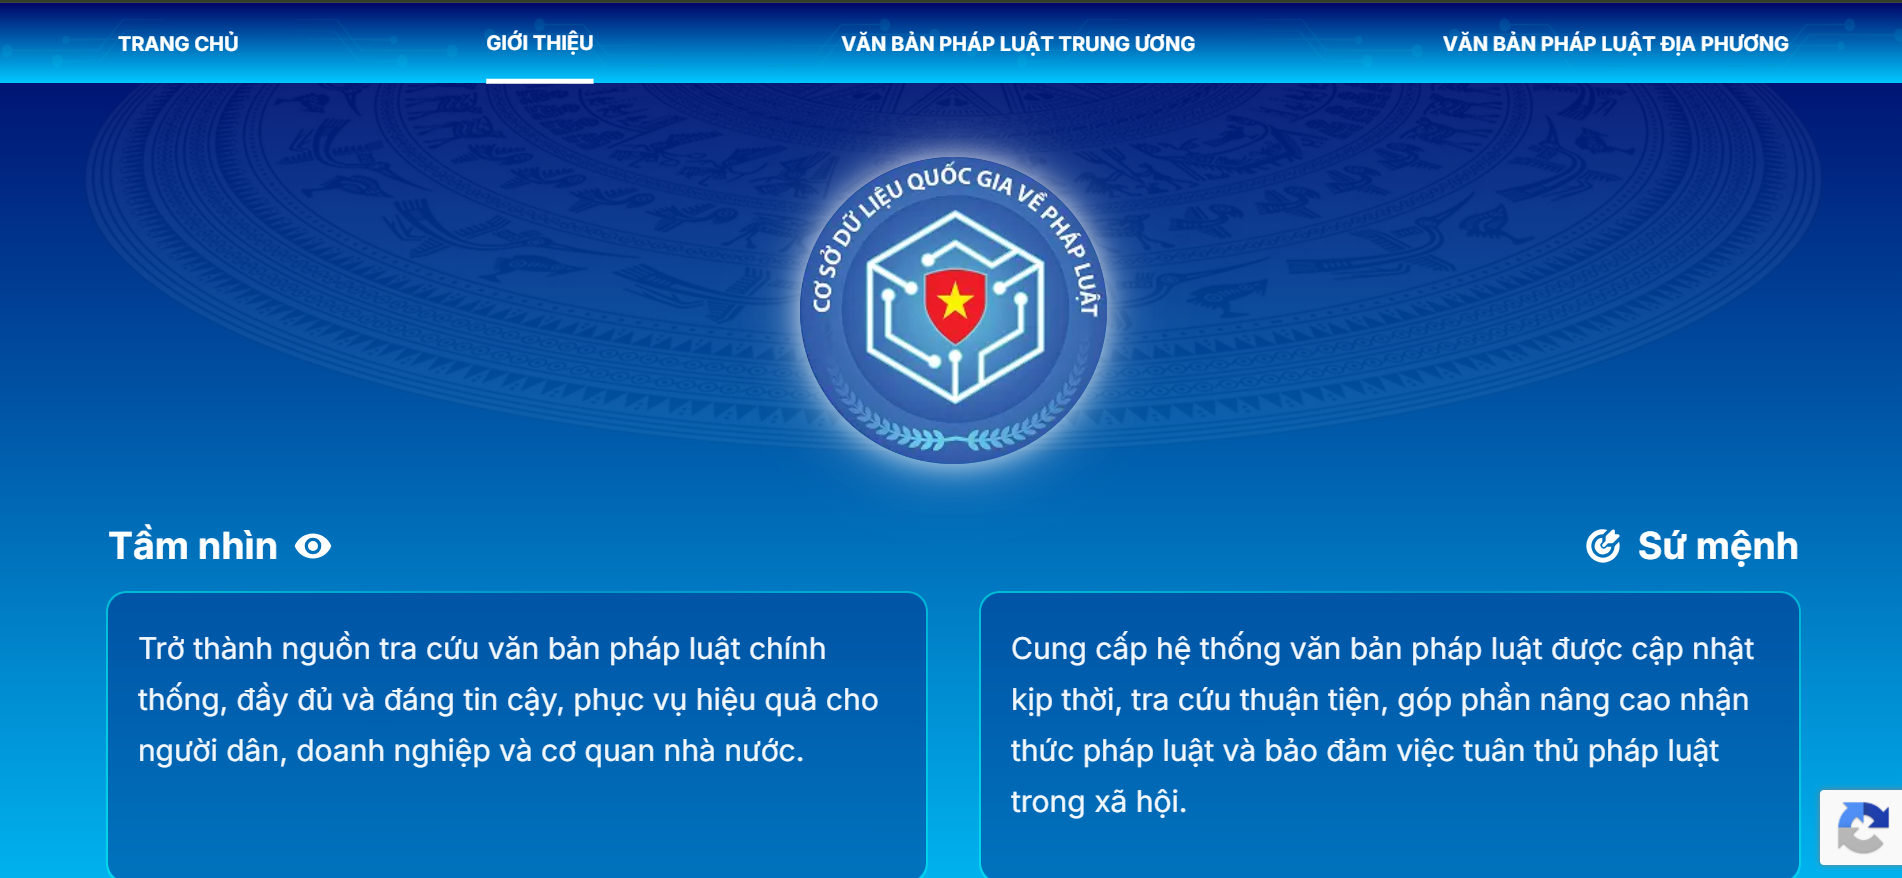
\includegraphics[scale = 0.2]{pictures/Home-vbpl.png}
\caption{Giao diện nguồn dữ liệu Văn bản pháp luật}
\end{figure}

Giao diện nguồn dữ liệu Pháp Điển


\begin{figure}[H]
\centering
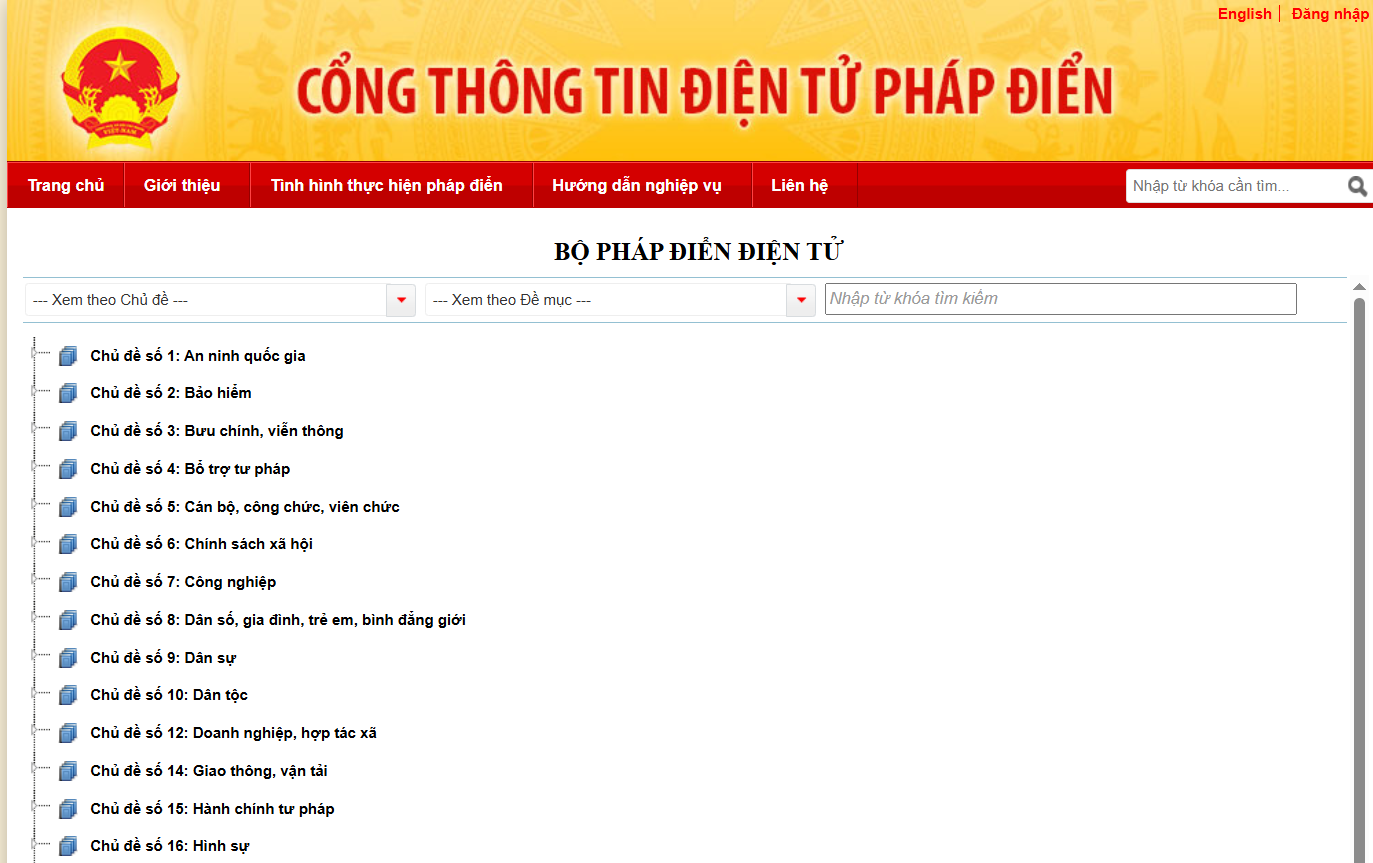
\includegraphics[scale = 0.3]{pictures/Home-PhapDien.png}
\caption{Giao diện nguồn dữ liệu Pháp Điển}
\end{figure}


Sơ đồ thu thập dữ liệu chung


\begin{figure}[H]
\centering
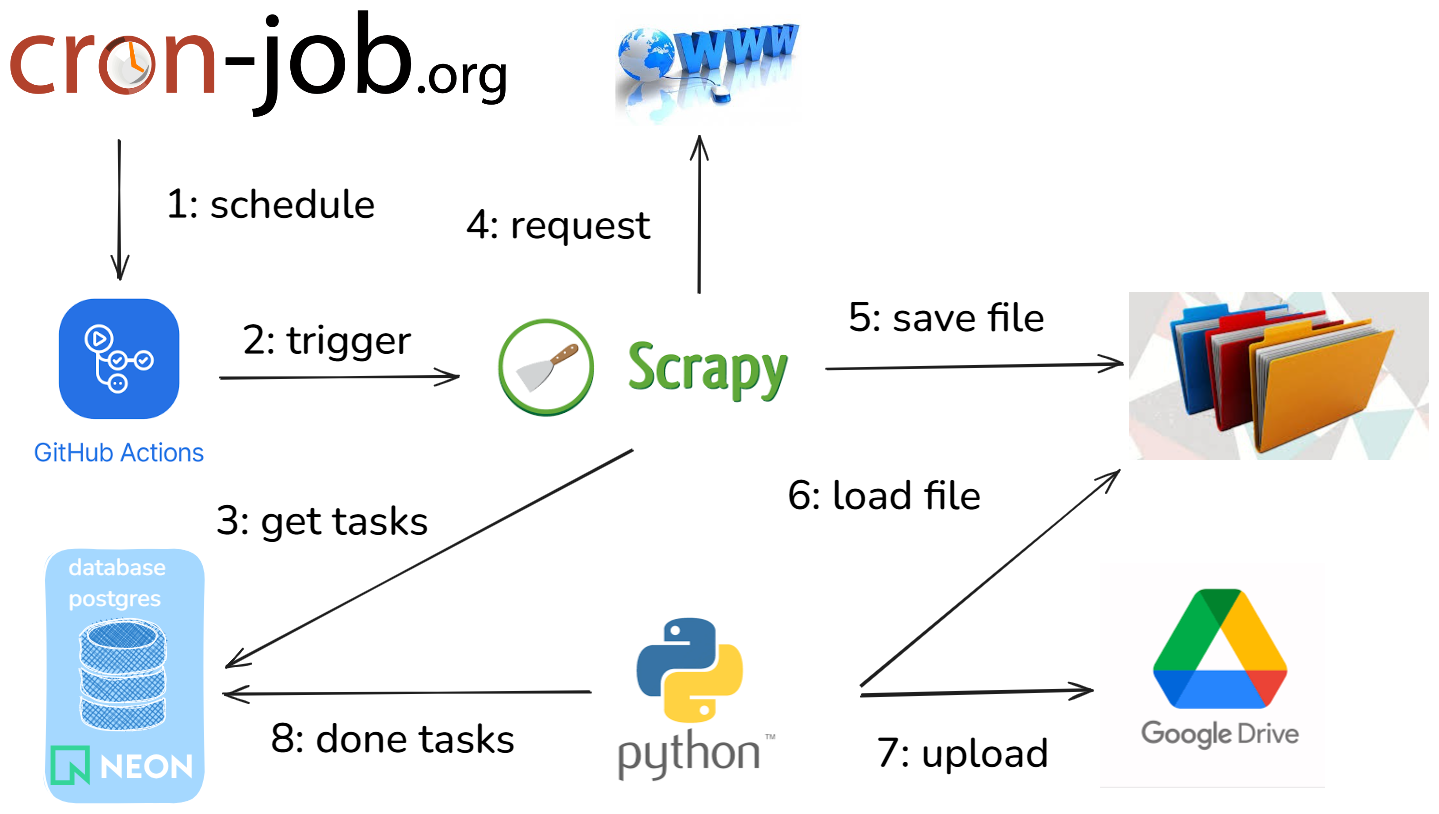
\includegraphics[scale = 0.2]{pictures/crawl-data.excalidraw.png}
\caption{Sơ đồ thu thập dữ liệu chung}
\end{figure}


Tại các bước sẽ sử dụng logic so sánh hash để bỏ qua văn bản không thay đổi nội dung
giúp tiết kiệm tài nguyên và thời gian xử lý dữ liệu.


% TODO: Có so sánh hash = tiết kiệm= nhanh


\begin{figure}[H]
\centering
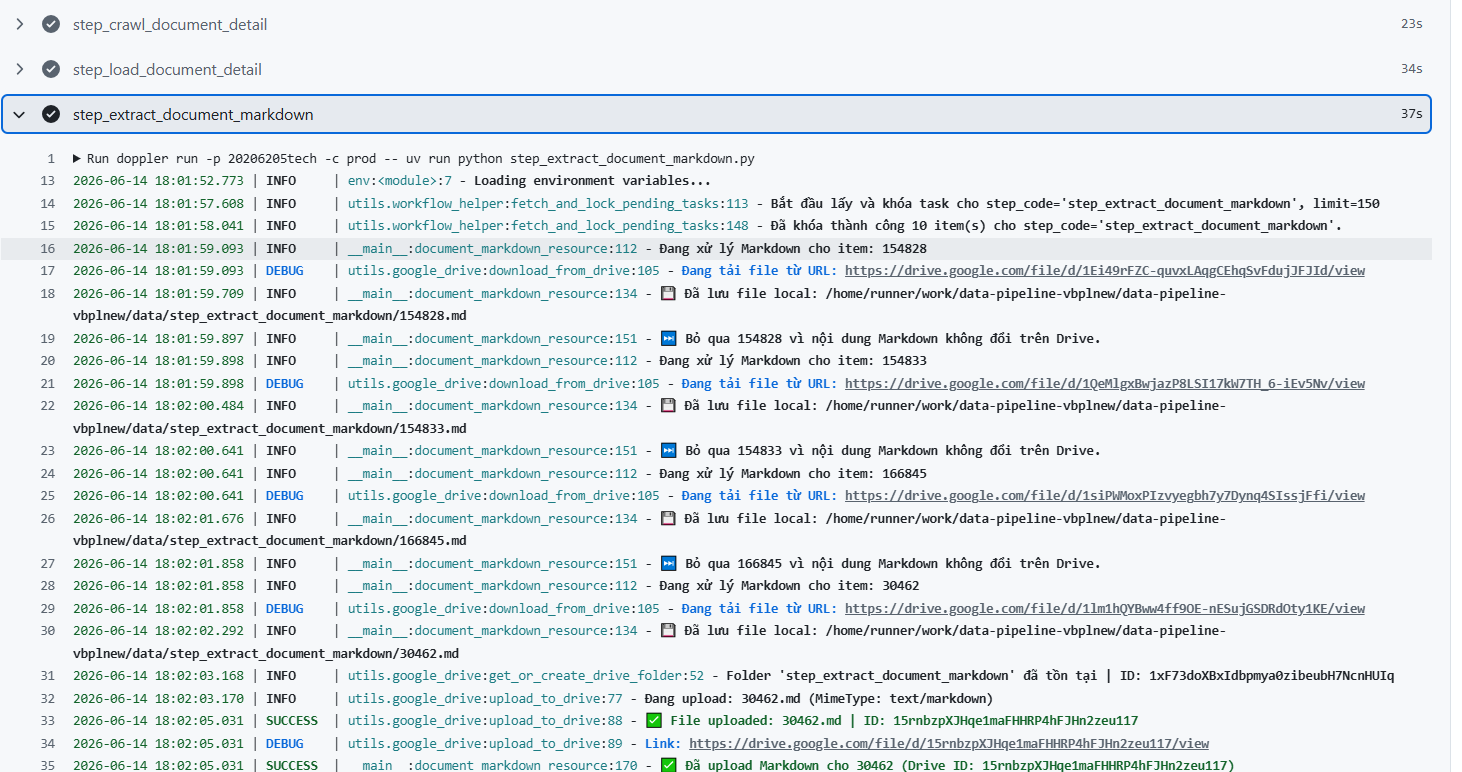
\includegraphics[scale = 0.2]{pictures/data-pipeline-hash-skip.png}
\caption{Sơ đồ thu thập dữ liệu chung}
\end{figure}

Thư viện dlt (Data Load Tool)
là một thư viện Python
mã nguồn mở
giúp trích xuất dữ liệu từ nhiều nguồn khác nhau
và tải chúng vào các tập dữ liệu có cấu trúc rõ ràng.


\begin{figure}[H]
\centering
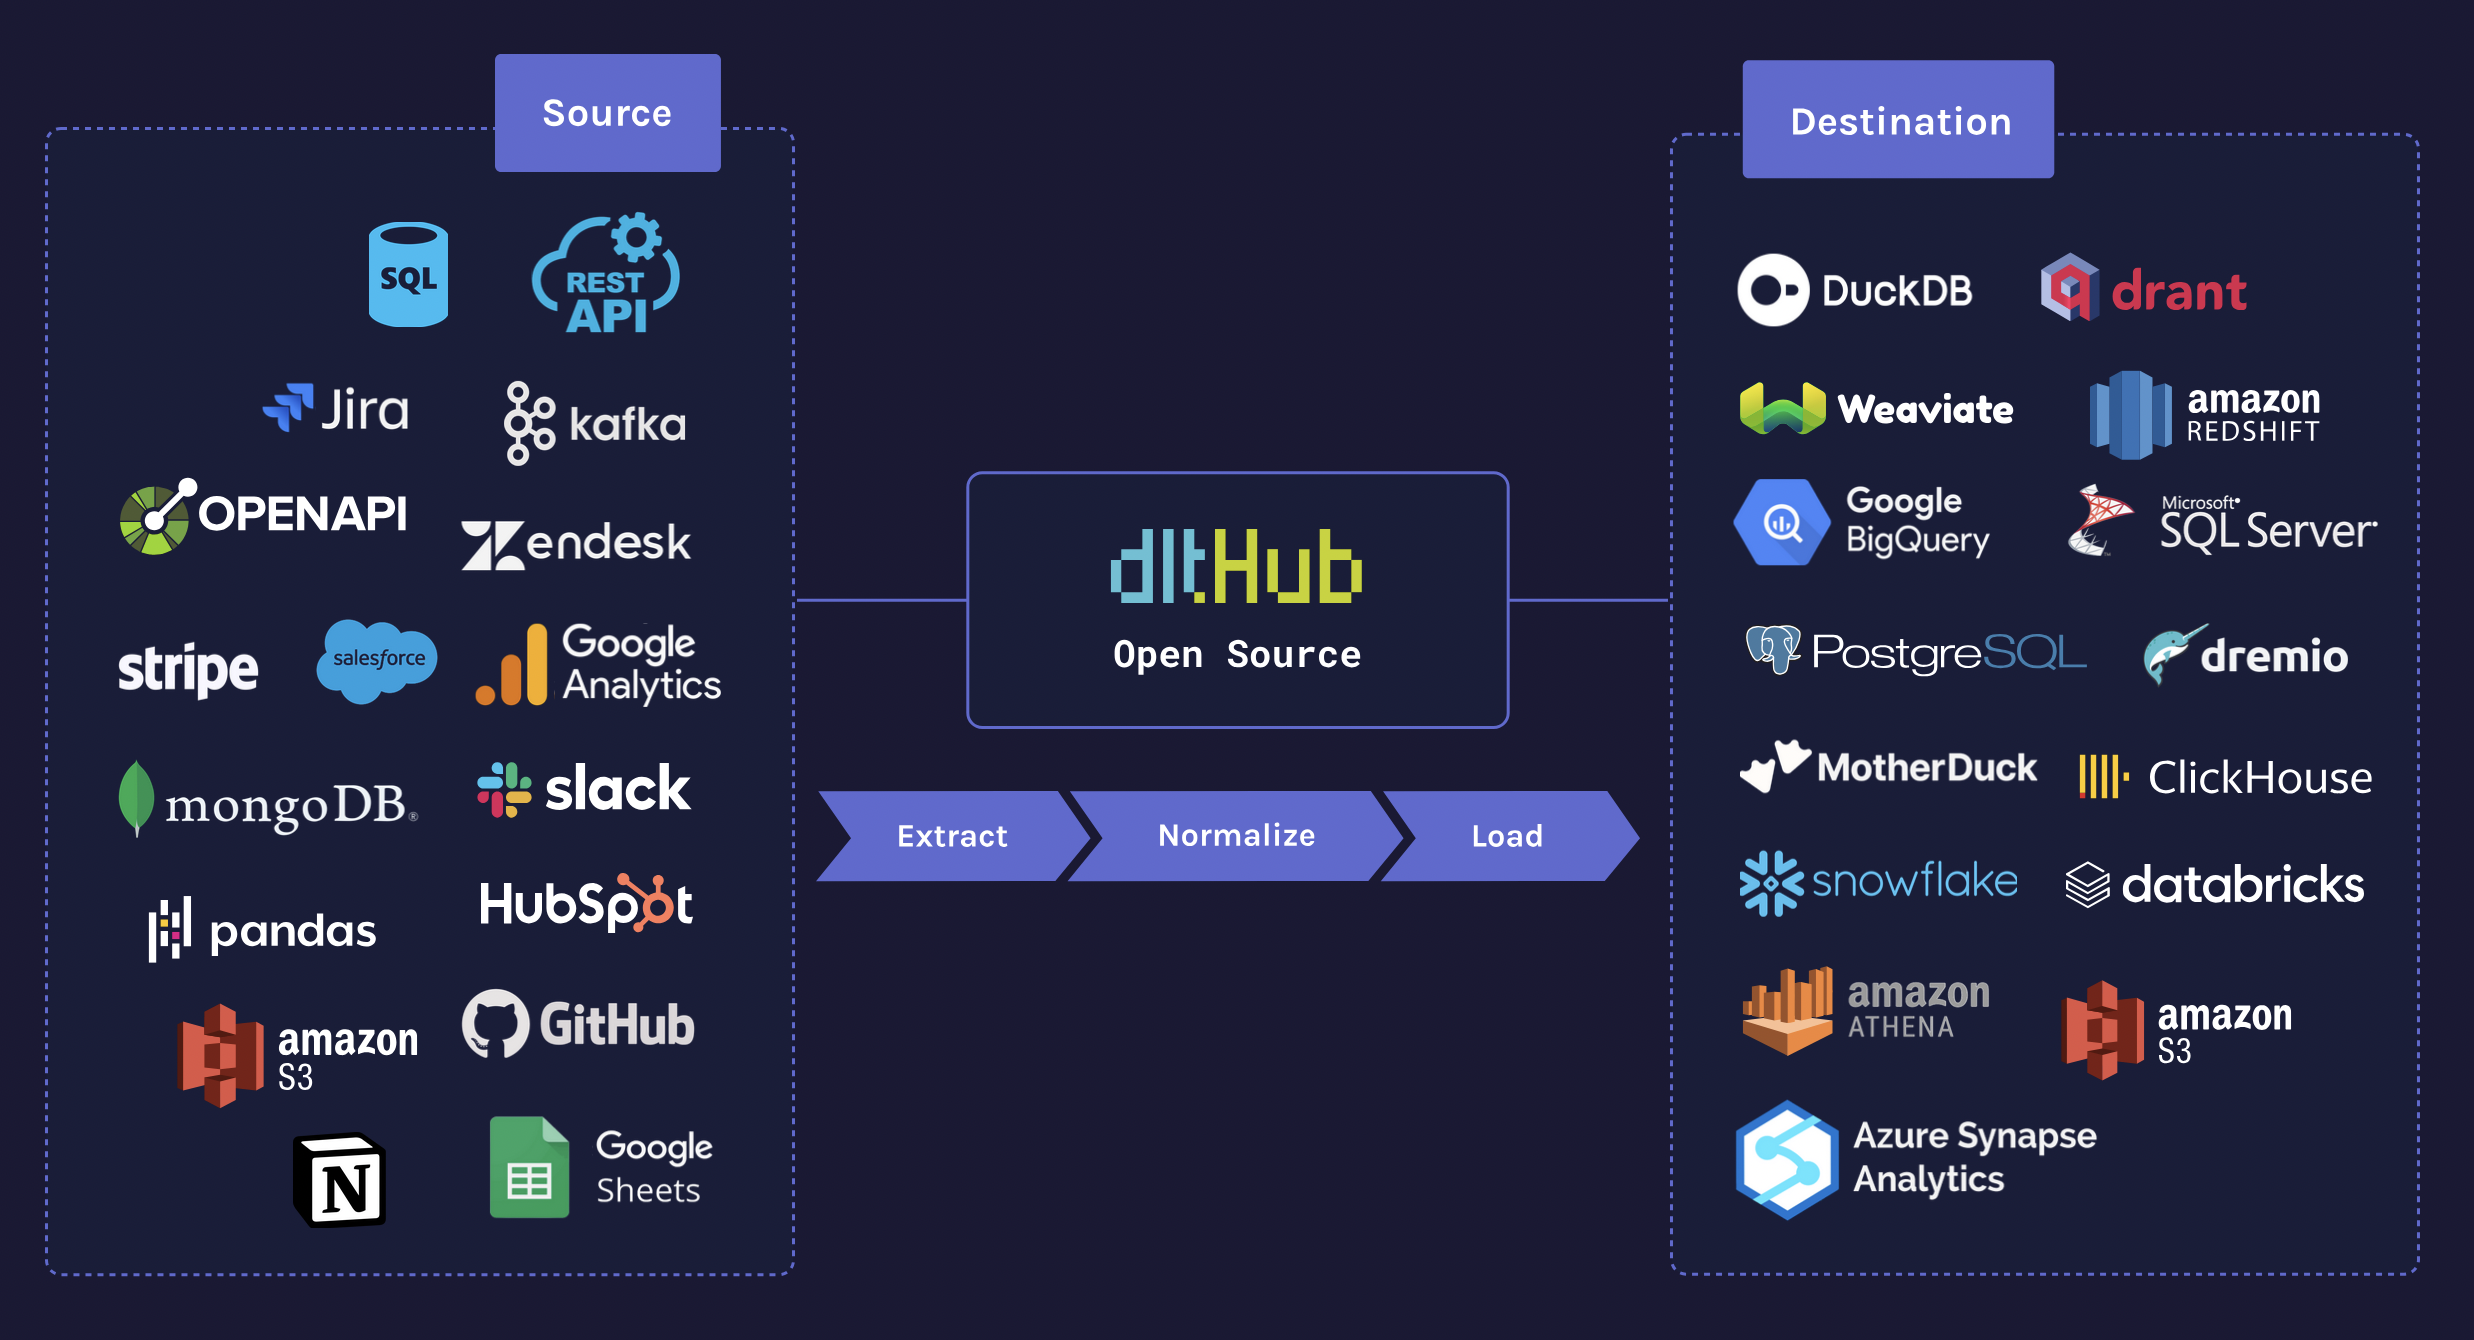
\includegraphics[scale = 0.2]{pictures/dlt-onepager-c61255330e30060ca8f2fa6d7b73b600.png}
\caption{Giao diện nguồn dữ liệu Văn bản pháp luật}
\end{figure}


Việc sử dụng Data Load Tool hỗ trợ
tự động nội suy cấu trúc, kiểu dữ liệu
và xử lý mượt mà các cấu trúc dữ liệu lồng nhau
hỗ trợ tốt việc thay đổi nếu
nguồn dữ liệu có sự thay đổi


\begin{figure}[H]
\centering
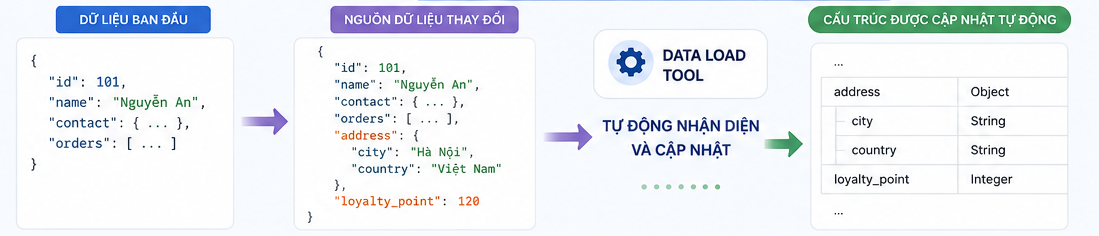
\includegraphics[scale = 0.2]{pictures/dlt-auto.png}
\caption{Data Load Tool tự động thích ứng nguồn dữ liệu có sự thay đổi}
\end{figure}


\subsubsection{Đường ống dữ liệu Văn bản pháp luật}


Khi làm việc với bài toán dữ liệu thực tế, việc thu thập dữ liệu
có thách thức
phụ thuộc
vào nguồn
dữ liệu.
Vào ngày 24/05/2026, nguồn dữ liệu Văn bản pháp luật được thay đổi cả hệ thống, API và giao diện.
Do sự thay đổi lớn về dữ liệu thu thập
nên hệ thống cần xử lý lại các bước Data pipeline.

Giao diện nguồn dữ liệu Văn bản pháp luật mới

\begin{figure}[H]
\centering
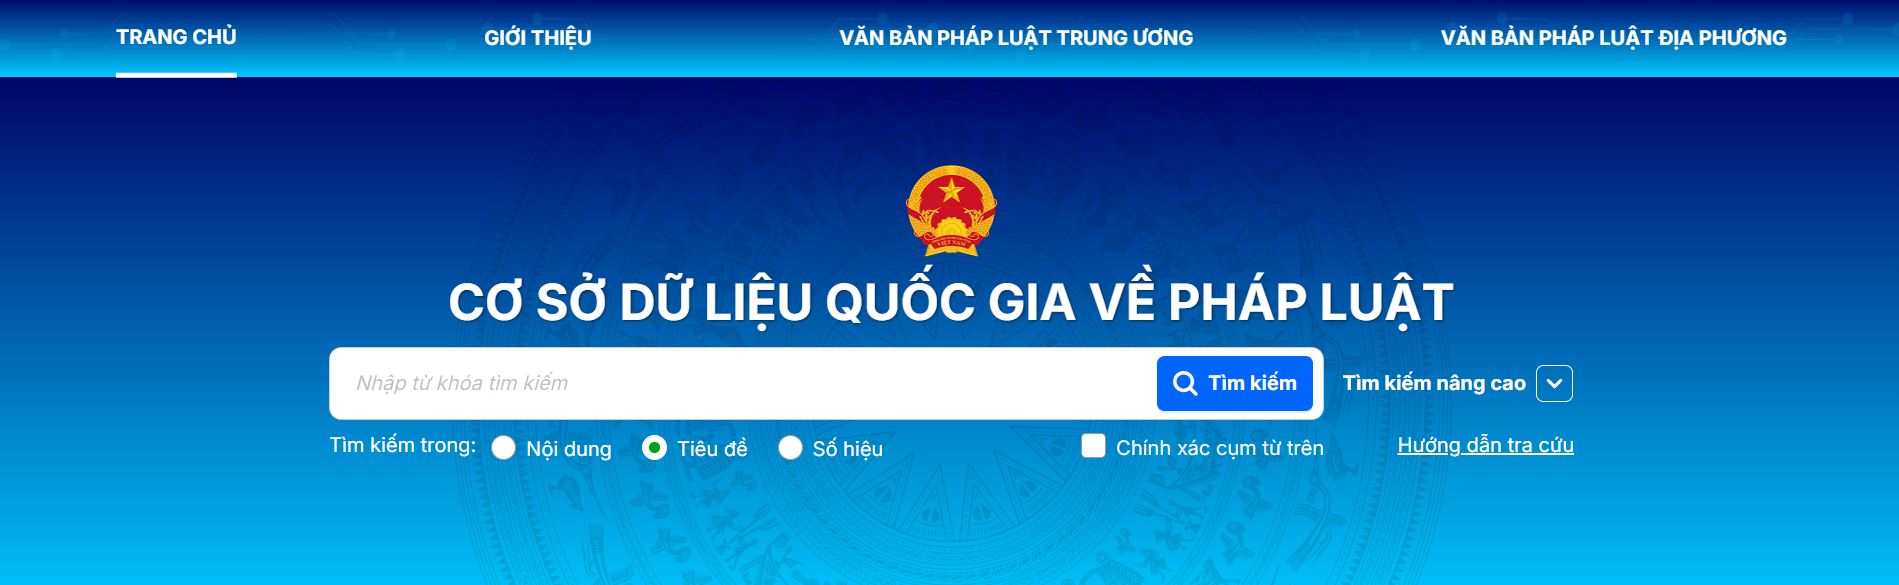
\includegraphics[scale = 0.2]{pictures/vbpl-search.png}
\caption{Sơ đồ thu thập dữ liệu chung}
\end{figure}


Sơ đồ tổng quan Data pipeline Văn bản pháp luật

\begin{figure}[H]
\centering
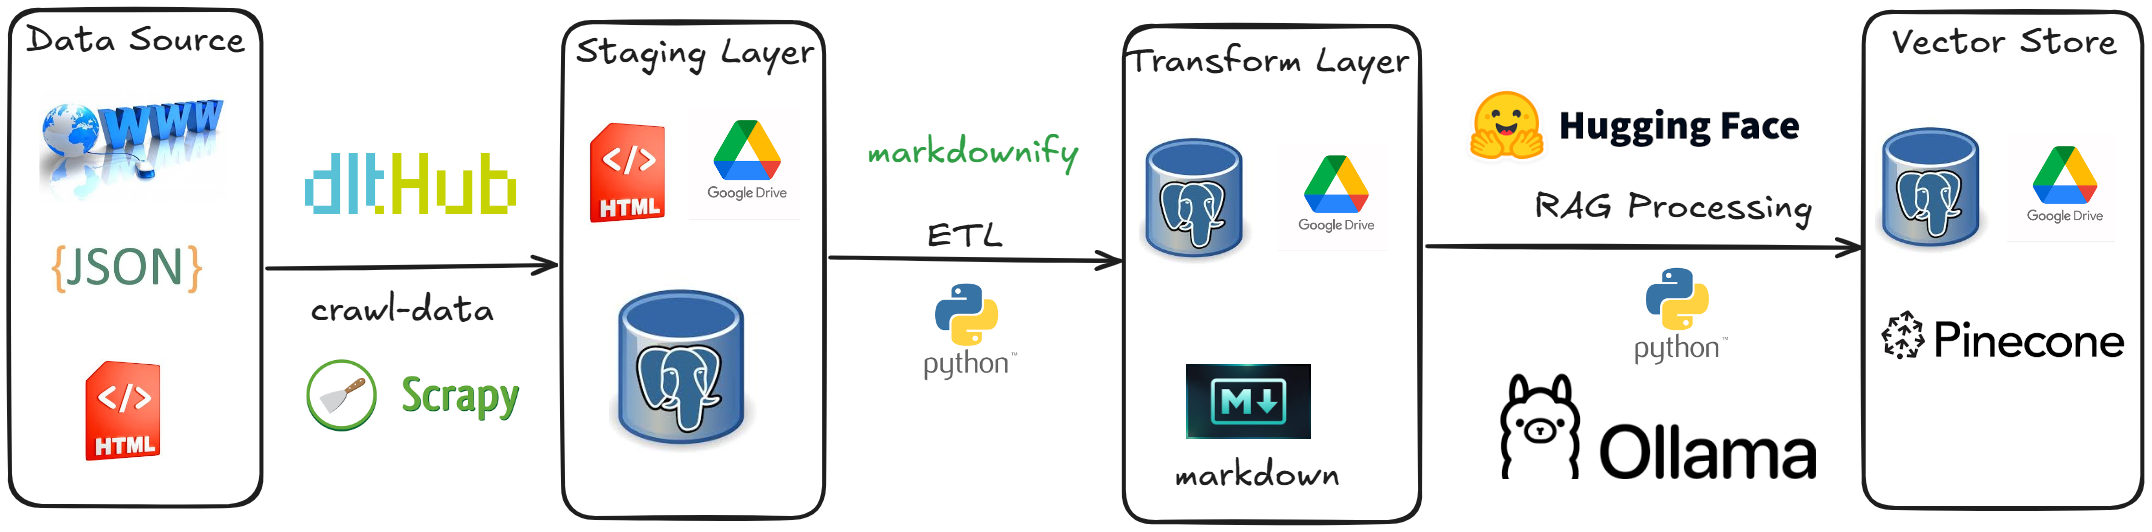
\includegraphics[scale = 0.2]{pictures/Data-Pipeline-VBPL.excalidraw.png}
\caption{Sơ đồ thu thập dữ liệu chung}
\end{figure}


Các bước thực hiện cũ

\begin{figure}[H]
\centering
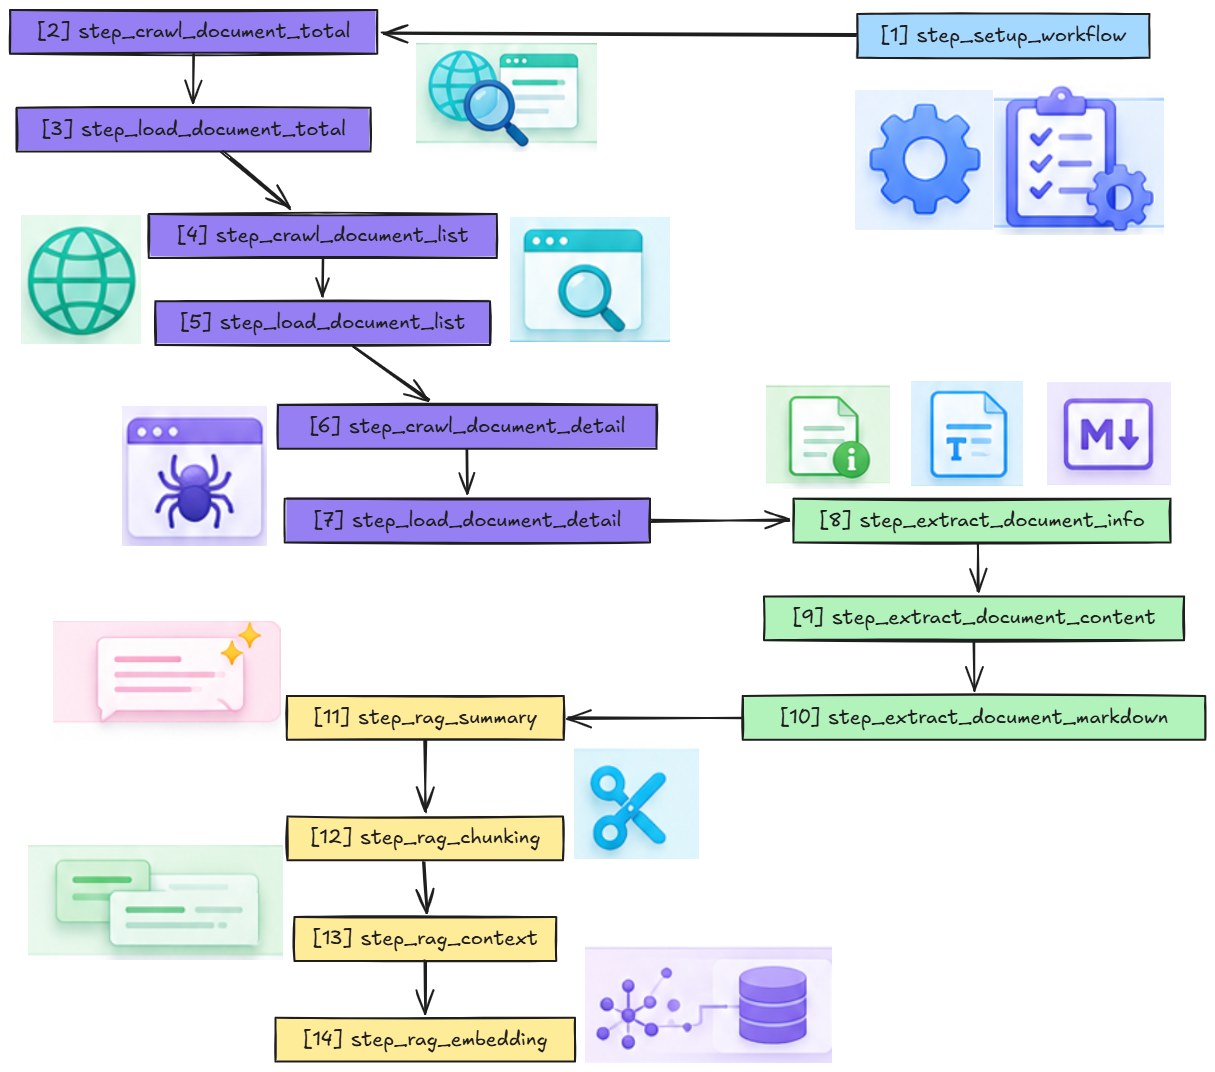
\includegraphics[scale = 0.2]{pictures/step0.excalidraw.png}
\caption{Sơ đồ thu thập dữ liệu chung}
\end{figure}


Mô tả các bước thực hiện cũ:

Quá trình Data pipeline được chia thành 3 giai đoạn: Thu thập dữ liệu, Tiền xử lý văn bản và Tích hợp RAG Pipeline.

\begin{itemize}


\item Giai đoạn Khởi tạo:
\begin{itemize}

\item step\_setup\_workflow cập nhật danh sách và thứ tự các bước (workflow) vào cơ sở dữ liệu PostgreSQL


\end{itemize}
\item Giai đoạn Thu thập Dữ liệu:
\begin{itemize}

\item step\_crawl\_document\_total và step\_load\_document\_total: thu thập tổng số lượng văn bản pháp luật hiện có trên hệ thống web.
\item step\_crawl\_document\_list và step\_load\_document\_list: Dựa vào sự chênh lệch tổng số lượng, tính toán số trang cần quét và thu thập danh sách các item\_id.
\item step\_crawl\_document\_detail và step\_load\_document\_detail: tải toàn bộ mã nguồn HTML trang chi tiết của từng văn bản và Upload các file HTML gốc này lên Google Drive, đồng thời lưu drive\_id và mã băm MD5 hash vào database để quản lý thay đổi.


\end{itemize}
\item Giai đoạn Tiền xử lý Dữ liệu:
\begin{itemize}

\item step\_extract\_document\_info: từ file HTML, bóc tách các siêu dữ liệu quan trọng (Metadata) như: Số hiệu, Cơ quan ban hành, Ngày có hiệu lực, Người ký, v.v., và lưu vào database.
\item step\_extract\_document\_content: Làm sạch file HTML, cắt bỏ các phần thừa (header, footer, menu) và chỉ giữ lại phần nội dung (thẻ div\#toanvancontent ).
\item step\_extract\_document\_markdown: Chuyển đổi file HTML đã làm sạch sang định dạng Markdown.


\end{itemize}
\item Giai đoạn Tích hợp RAG pipeline
\begin{itemize}

\item step\_rag\_summary: Sử dụng LLM viết một bản tóm tắt ngắn gọn mô tả bức tranh toàn cảnh của văn bản pháp luật đó.
\item step\_rag\_chunking: Chạy Semantic Chunking. LLM sẽ dựa vào bản tóm tắt và nội dung chi tiết để quyết định các "điểm cắt" tối ưu, chia nhỏ văn bản thành các đoạn (chunks) sao cho không bị đứt gãy ý nghĩa.
\item step\_rag\_context: Đây là bước chống mất ngữ cảnh. LLM sẽ sinh ra ngữ cảnh cho từng đoạn chunk nhỏ vừa được cắt, đảm bảo mỗi chunk đều có thể đứng độc lập khi được tìm kiếm.
\item step\_rag\_embedding: Sử dụng mô hình HuggingFace ( keepitreal/vietnamese-sbert ) để biến đổi các đoạn văn bản (đã có ngữ cảnh) thành vector đa chiều và lưu trữ vào VectorDB (Pinecone).
\end{itemize}
\end{itemize}


Các bước thực hiện mới

\begin{figure}[H]
\centering
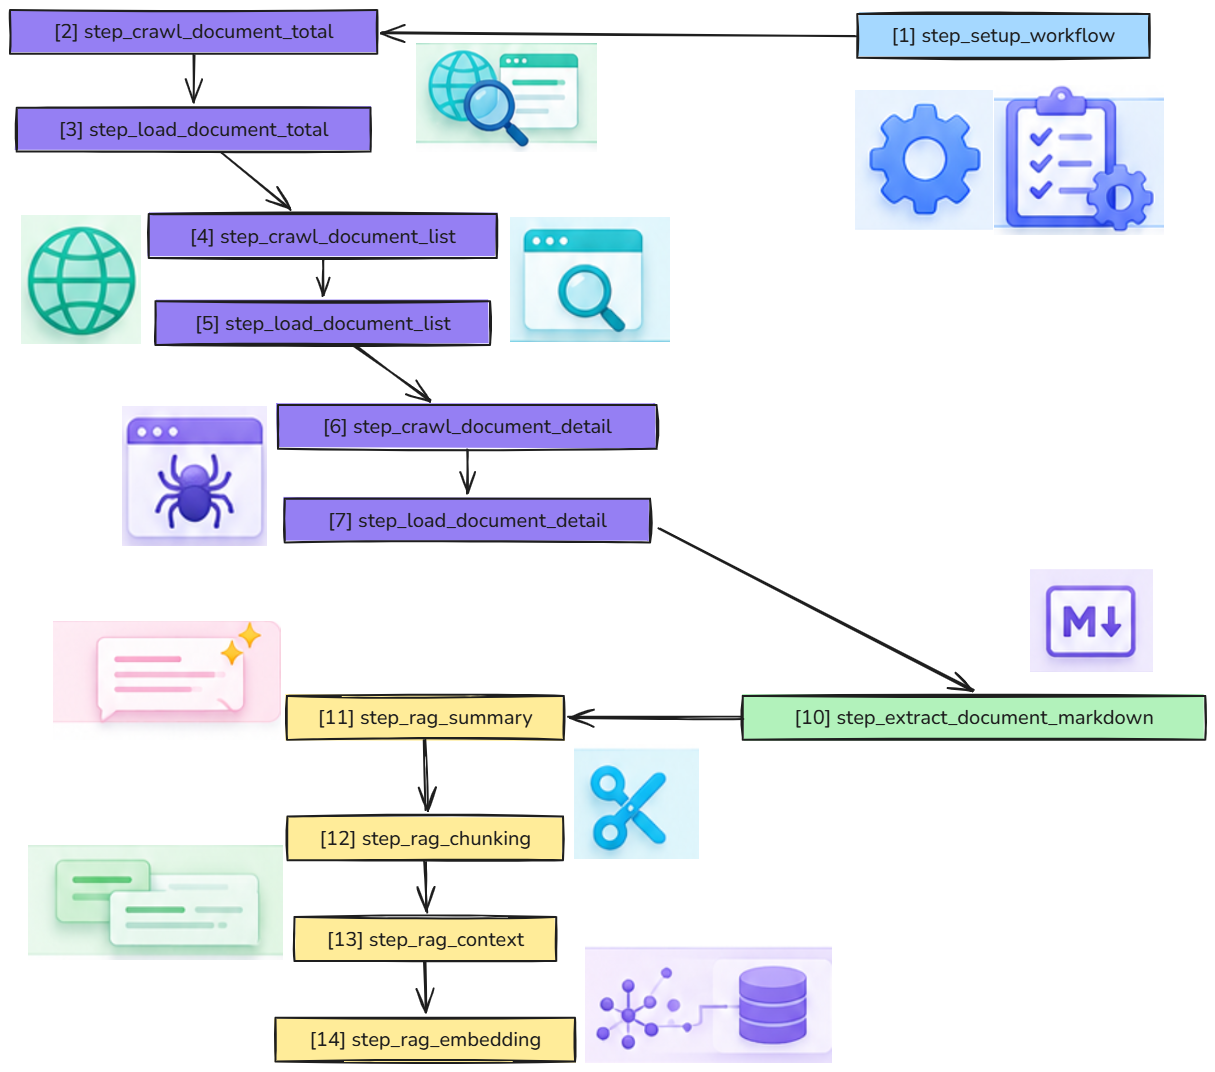
\includegraphics[scale = 0.2]{pictures/step1.excalidraw.png}
\caption{Sơ đồ thu thập dữ liệu chung}
\end{figure}


\begin{itemize}
\item Nhờ vào việc nguồn dữ liệu thay đổi sang hệ thống API mới
trả về cấu trúc JSON giàu thông tin, hệ thống không còn cần các bước bóc tách thủ công từ mã nguồn HTML phức tạp, giúp tăng tốc độ xử lý và độ chính xác của dữ liệu.

\item Hệ thống loại bỏ bước step\_extract\_document\_info vì nội dung Metadata chi tiết đã có trong API

\item Hệ thống loại bỏ bước step\_extract\_document\_content vì nội dung văn bản đã được API trả trong thông tin documentContent


\end{itemize}


\begin{figure}[H]
\centering
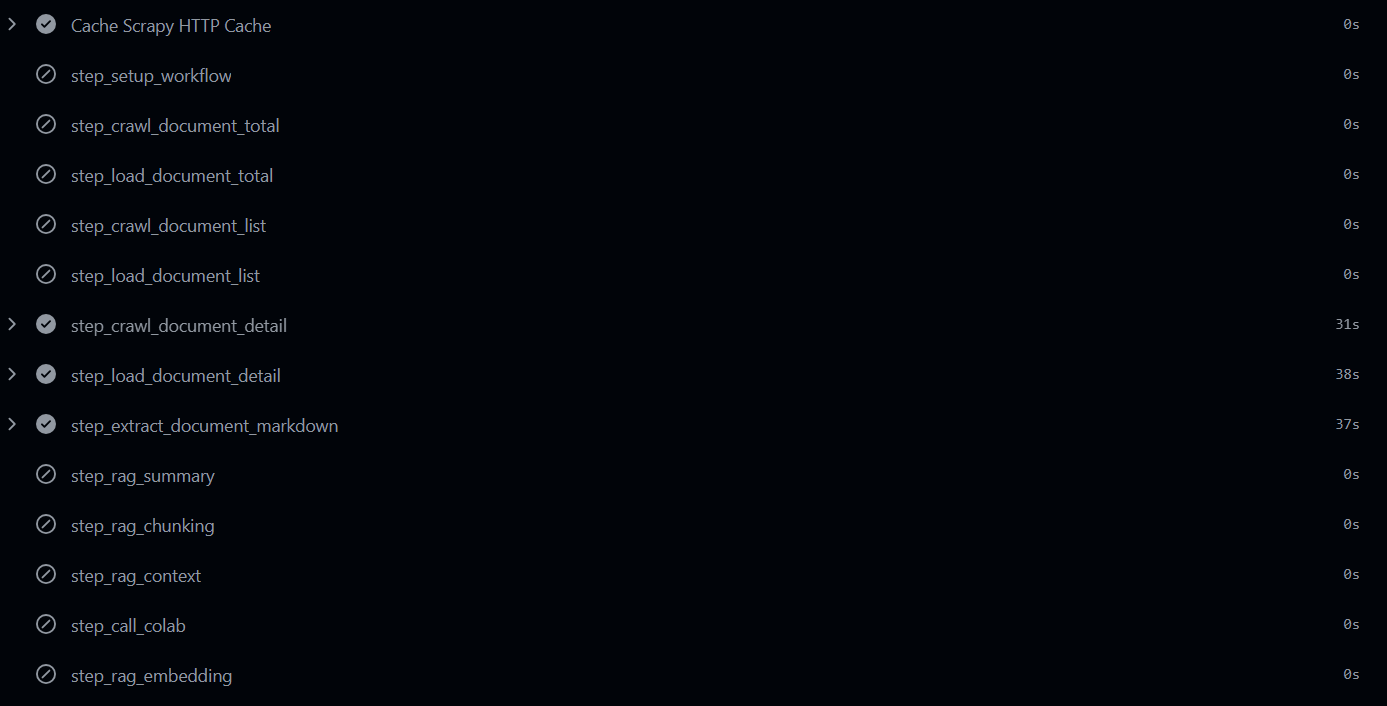
\includegraphics[scale = 0.2]{pictures/github-action-vbpl.png}
\caption{Sơ đồ thu thập dữ liệu chung}
\end{figure}


\subsubsection{Đường ống dữ liệu Pháp Điển}

Pháp điển là tập hợp các quy phạm pháp luật đang còn hiệu lực của các văn bản quy phạm pháp luật do cơ quan nhà nước ở trung ương ban hành, từ Thông tư trở lên và trừ Hiến pháp.

Sơ đồ tổng quan Data pipeline Pháp Điển


\begin{figure}[H]
\centering
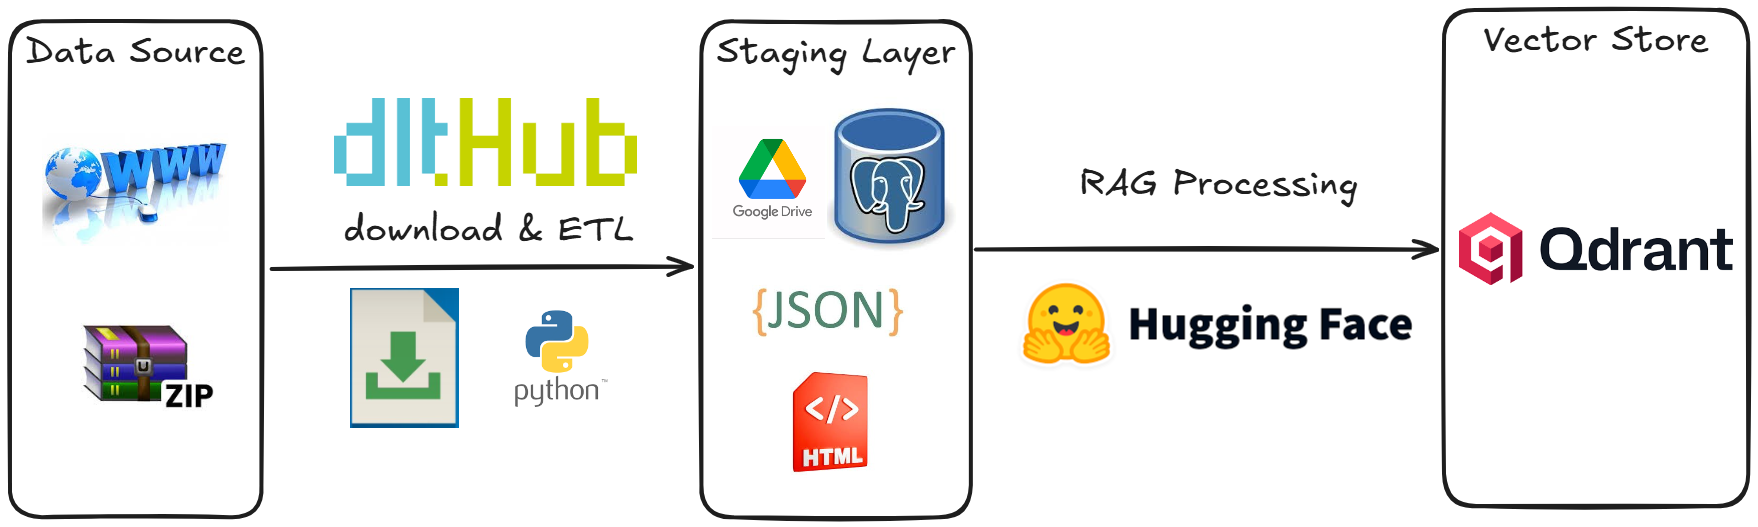
\includegraphics[scale = 0.2]{pictures/Data-Pipeline-PhapDien.excalidraw.png}
\caption{Sơ đồ thu thập dữ liệu chung}
\end{figure}


Tổng quan thông tin file zip


\begin{figure}[H]
\centering
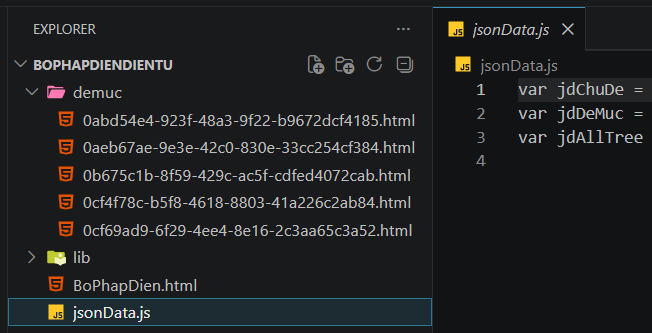
\includegraphics[scale = 0.2]{pictures/zip_file_PhapDien.png}
\caption{Sơ đồ thu thập dữ liệu chung}
\end{figure}


Kết quả file JSON đã trích xuất


\begin{figure}[H]
\centering
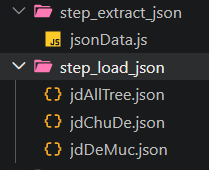
\includegraphics[scale = 0.2]{pictures/step_json_PhapDien.png}
\caption{Sơ đồ thu thập dữ liệu chung}
\end{figure}


Kết quả vector được lưu trong vector database


\begin{figure}[H]
\centering
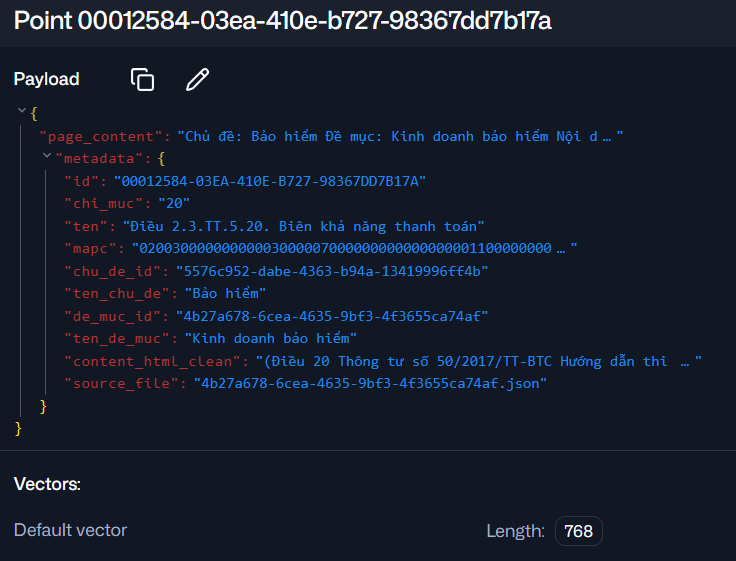
\includegraphics[scale = 0.2]{pictures/vector_database_PhapDien.png}
\caption{Sơ đồ thu thập dữ liệu chung}
\end{figure}


Các bước thực hiện


\begin{figure}[H]
\centering
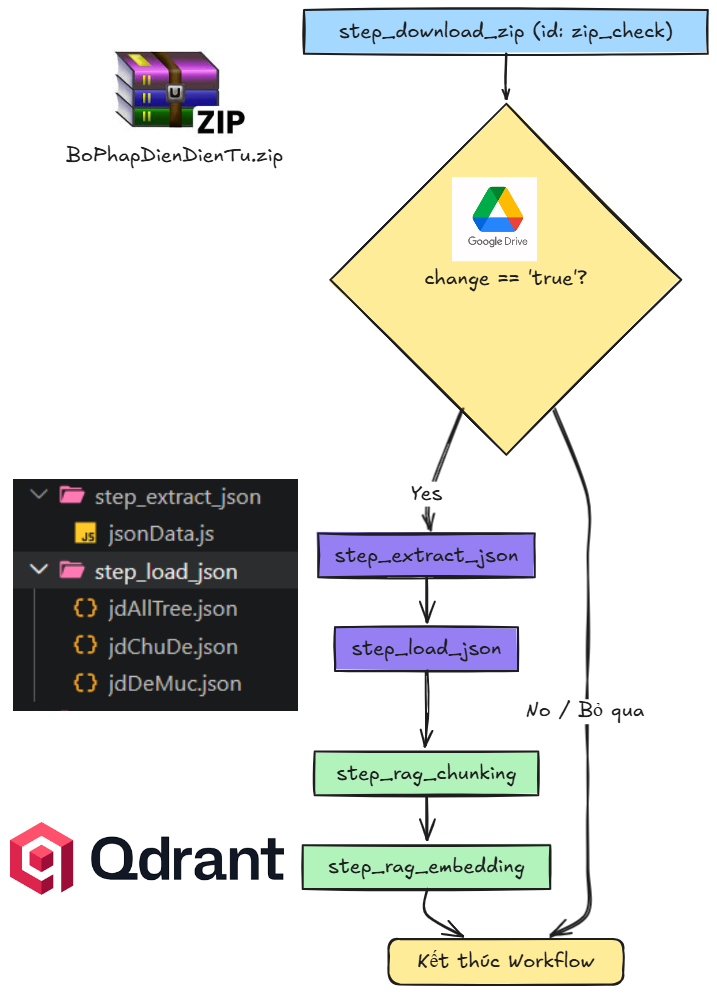
\includegraphics[scale = 0.2]{pictures/step3.excalidraw.png}
\caption{Sơ đồ thu thập dữ liệu chung}
\end{figure}


Mô tả các bước thực hiện:

Quá trình Data pipeline được chia thành 3 giai đoạn: Thu thập dữ liệu, Tiền xử lý văn bản và Tích hợp RAG Pipeline.

- Giai đoạn Thu thập Dữ liệu:

- step\_download\_zip: Tự động tải file nén chứa toàn bộ Bộ pháp điển điện tử ( BoPhapDienDienTu.zip ) từ nguồn Cổng thông tin điện tử pháp điển. Hệ thống tính toán mã băm (MD5) và đồng bộ với Google Drive để kiểm tra sự thay đổi dữ liệu.

- Giai đoạn Tiền xử lý Dữ liệu:

- step\_extract\_json và step\_load\_json: Từ file jsonData.js. Tiến hành bóc tách (parse) các biến cấu trúc dữ liệu để lấy danh sách Chủ đề (jdChuDe), Đề mục (jdDeMuc), và Cây mục lục (jdAllTree), sau đó xuất ra định dạng JSON.

- Giai đoạn Tích hợp RAG Pipeline:

- step\_rag\_chunking: Thực hiện đối chiếu từ Cây mục lục (jdAllTree) với các thẻ bên trong từng file HTML chi tiết. Từ đó, bóc tách chính xác từng phần nội dung văn bản thành dạng JSON có các đoạn văn bản và siêu dữ liệu (Metadata).

- step\_rag\_embedding: Làm giàu ngữ cảnh bằng cách nối trực tiếp tên Chủ đề và Đề mục vào phần đầu của mỗi đoạn văn bản chunk. Sau đó, nội dung được đưa qua mô hình HuggingFace ( keepitreal/vietnamese-sbert ) để biến đổi thành các vector cơ sở dữ liệu vector Qdrant.


\begin{figure}[H]
\centering
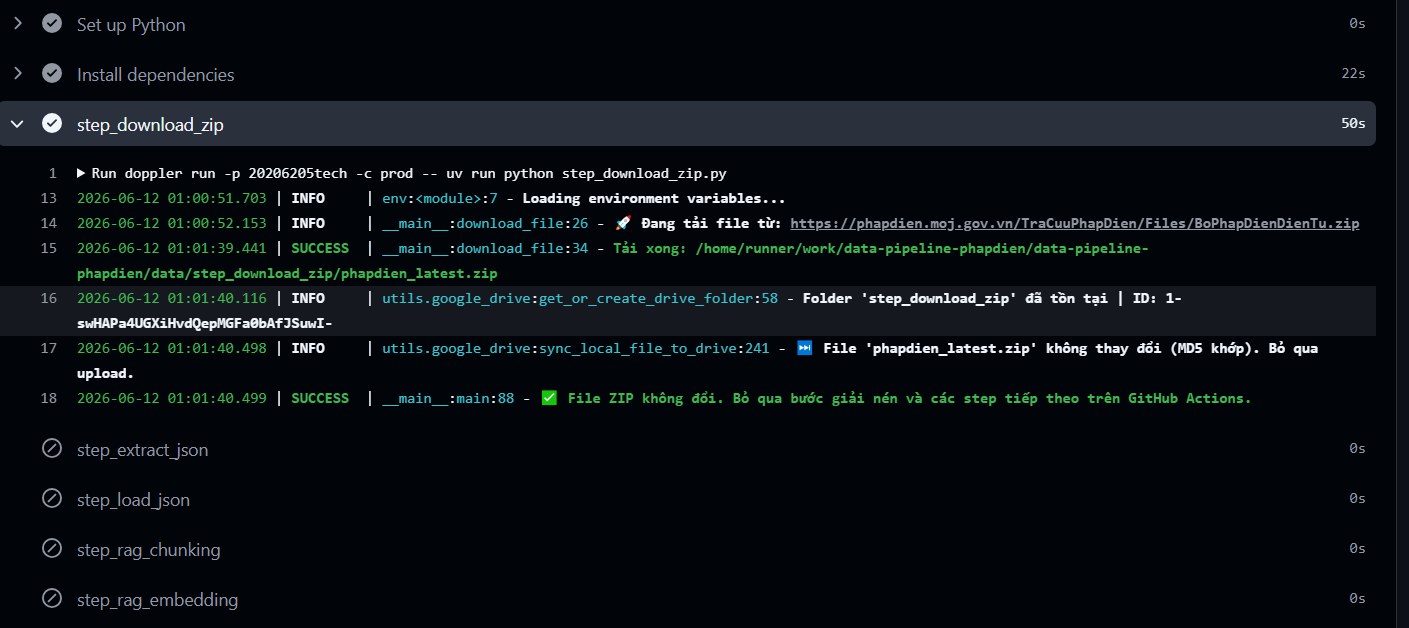
\includegraphics[scale = 0.2]{pictures/github-action-PhapDien.png}
\caption{Sơ đồ thu thập dữ liệu chung}
\end{figure}


\begin{figure}[H]
\centering
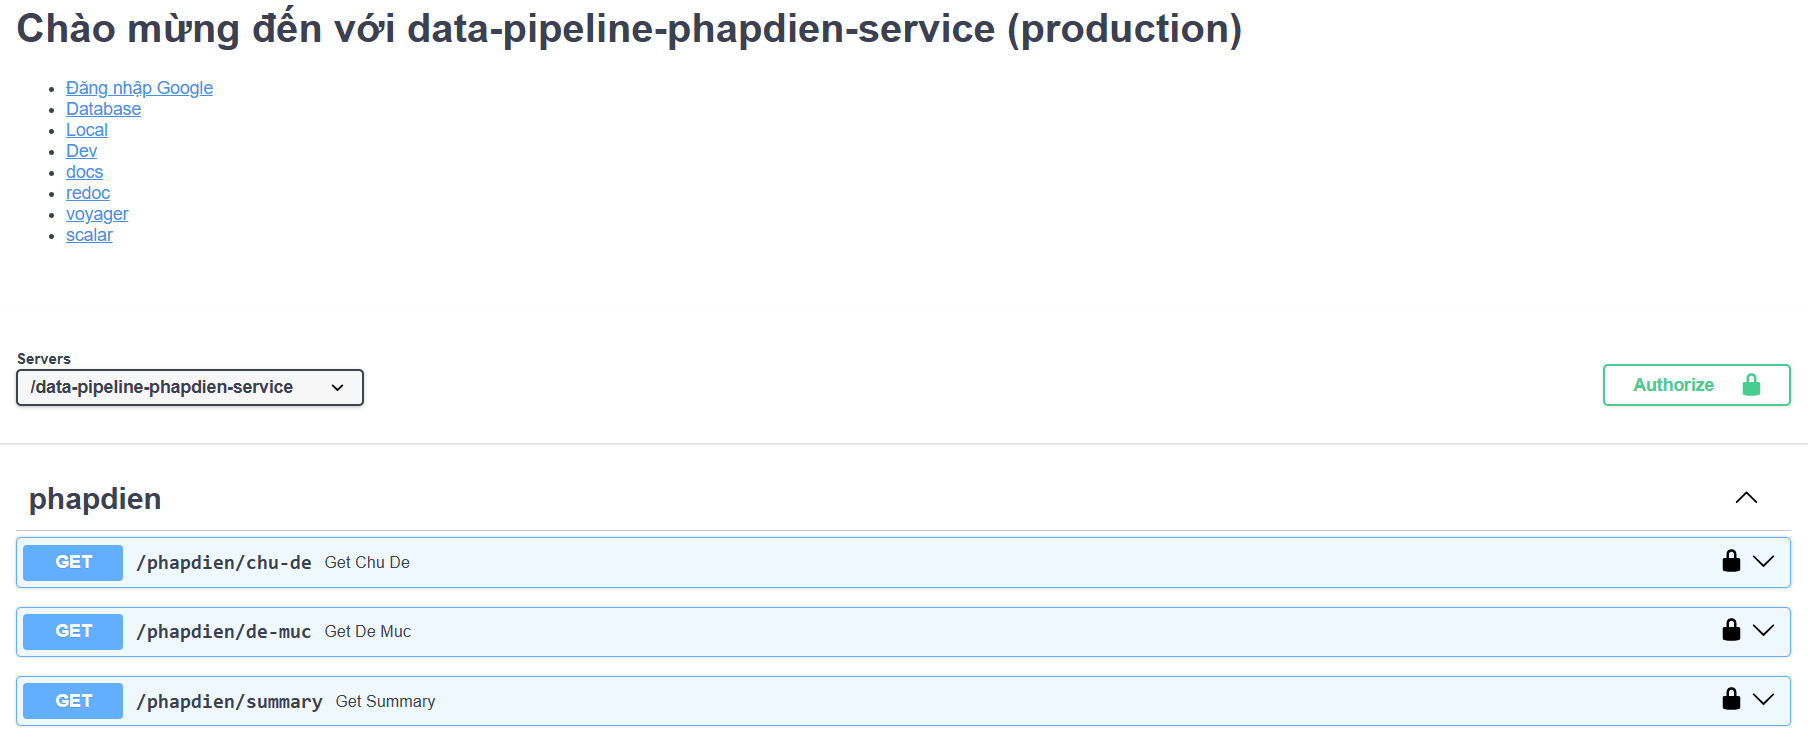
\includegraphics[scale = 0.2]{pictures/PhapDien-SERVICE.png}
\caption{swagger}
\end{figure}

\begin{figure}[H]
\centering
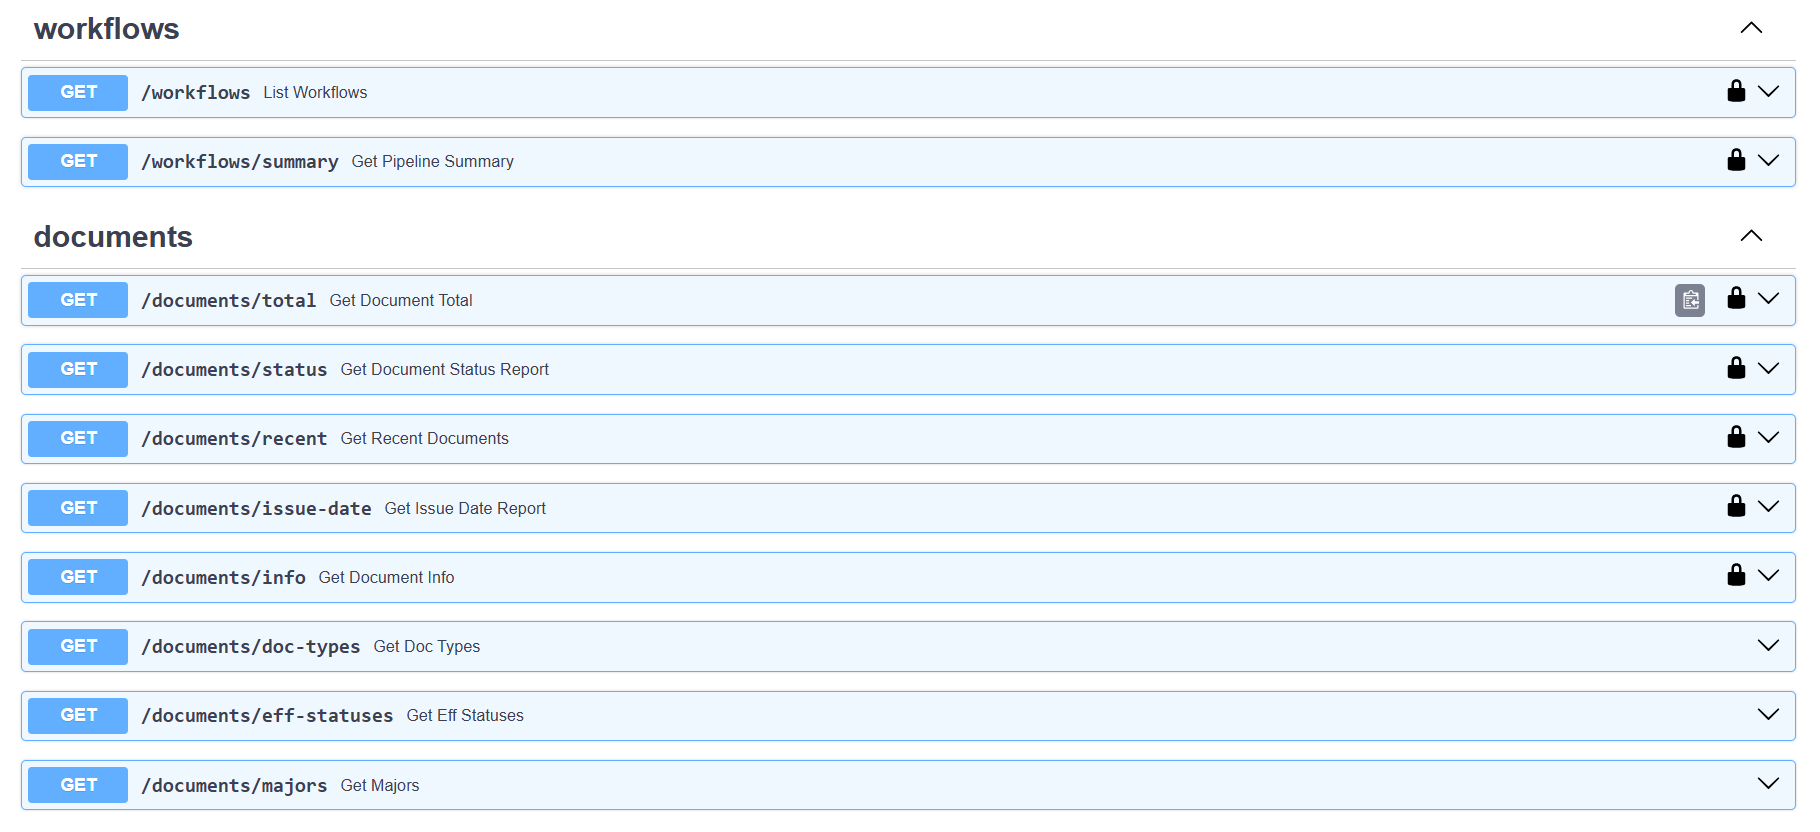
\includegraphics[scale = 0.2]{pictures/VBPL-SERVICE.png}
\caption{swagger}
\end{figure}


\begin{figure}[H]
\centering
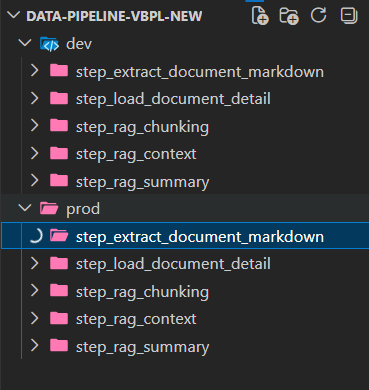
\includegraphics[scale = 0.2]{pictures/google-drive-VBPL.png}
\caption{swagger}
\end{figure}
\begin{figure}[H]
\centering
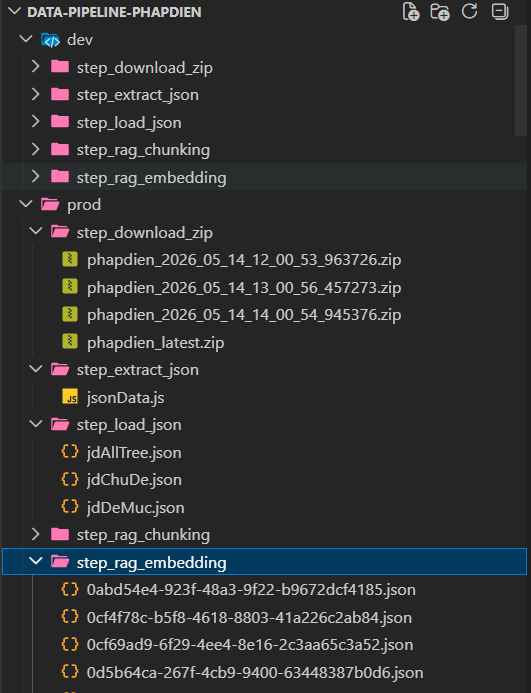
\includegraphics[scale = 0.2]{pictures/google-drive-PhapDien.png}
\caption{swagger}
\end{figure}
